% Options for packages loaded elsewhere
\PassOptionsToPackage{unicode}{hyperref}
\PassOptionsToPackage{hyphens}{url}
\PassOptionsToPackage{dvipsnames,svgnames,x11names}{xcolor}
%
\documentclass[
  letterpaper,
  DIV=11,
  numbers=noendperiod]{scrreprt}

\usepackage{amsmath,amssymb}
\usepackage{iftex}
\ifPDFTeX
  \usepackage[T1]{fontenc}
  \usepackage[utf8]{inputenc}
  \usepackage{textcomp} % provide euro and other symbols
\else % if luatex or xetex
  \usepackage{unicode-math}
  \defaultfontfeatures{Scale=MatchLowercase}
  \defaultfontfeatures[\rmfamily]{Ligatures=TeX,Scale=1}
\fi
\usepackage{lmodern}
\ifPDFTeX\else  
    % xetex/luatex font selection
\fi
% Use upquote if available, for straight quotes in verbatim environments
\IfFileExists{upquote.sty}{\usepackage{upquote}}{}
\IfFileExists{microtype.sty}{% use microtype if available
  \usepackage[]{microtype}
  \UseMicrotypeSet[protrusion]{basicmath} % disable protrusion for tt fonts
}{}
\makeatletter
\@ifundefined{KOMAClassName}{% if non-KOMA class
  \IfFileExists{parskip.sty}{%
    \usepackage{parskip}
  }{% else
    \setlength{\parindent}{0pt}
    \setlength{\parskip}{6pt plus 2pt minus 1pt}}
}{% if KOMA class
  \KOMAoptions{parskip=half}}
\makeatother
\usepackage{xcolor}
\setlength{\emergencystretch}{3em} % prevent overfull lines
\setcounter{secnumdepth}{5}
% Make \paragraph and \subparagraph free-standing
\ifx\paragraph\undefined\else
  \let\oldparagraph\paragraph
  \renewcommand{\paragraph}[1]{\oldparagraph{#1}\mbox{}}
\fi
\ifx\subparagraph\undefined\else
  \let\oldsubparagraph\subparagraph
  \renewcommand{\subparagraph}[1]{\oldsubparagraph{#1}\mbox{}}
\fi

\usepackage{color}
\usepackage{fancyvrb}
\newcommand{\VerbBar}{|}
\newcommand{\VERB}{\Verb[commandchars=\\\{\}]}
\DefineVerbatimEnvironment{Highlighting}{Verbatim}{commandchars=\\\{\}}
% Add ',fontsize=\small' for more characters per line
\usepackage{framed}
\definecolor{shadecolor}{RGB}{241,243,245}
\newenvironment{Shaded}{\begin{snugshade}}{\end{snugshade}}
\newcommand{\AlertTok}[1]{\textcolor[rgb]{0.68,0.00,0.00}{#1}}
\newcommand{\AnnotationTok}[1]{\textcolor[rgb]{0.37,0.37,0.37}{#1}}
\newcommand{\AttributeTok}[1]{\textcolor[rgb]{0.40,0.45,0.13}{#1}}
\newcommand{\BaseNTok}[1]{\textcolor[rgb]{0.68,0.00,0.00}{#1}}
\newcommand{\BuiltInTok}[1]{\textcolor[rgb]{0.00,0.23,0.31}{#1}}
\newcommand{\CharTok}[1]{\textcolor[rgb]{0.13,0.47,0.30}{#1}}
\newcommand{\CommentTok}[1]{\textcolor[rgb]{0.37,0.37,0.37}{#1}}
\newcommand{\CommentVarTok}[1]{\textcolor[rgb]{0.37,0.37,0.37}{\textit{#1}}}
\newcommand{\ConstantTok}[1]{\textcolor[rgb]{0.56,0.35,0.01}{#1}}
\newcommand{\ControlFlowTok}[1]{\textcolor[rgb]{0.00,0.23,0.31}{#1}}
\newcommand{\DataTypeTok}[1]{\textcolor[rgb]{0.68,0.00,0.00}{#1}}
\newcommand{\DecValTok}[1]{\textcolor[rgb]{0.68,0.00,0.00}{#1}}
\newcommand{\DocumentationTok}[1]{\textcolor[rgb]{0.37,0.37,0.37}{\textit{#1}}}
\newcommand{\ErrorTok}[1]{\textcolor[rgb]{0.68,0.00,0.00}{#1}}
\newcommand{\ExtensionTok}[1]{\textcolor[rgb]{0.00,0.23,0.31}{#1}}
\newcommand{\FloatTok}[1]{\textcolor[rgb]{0.68,0.00,0.00}{#1}}
\newcommand{\FunctionTok}[1]{\textcolor[rgb]{0.28,0.35,0.67}{#1}}
\newcommand{\ImportTok}[1]{\textcolor[rgb]{0.00,0.46,0.62}{#1}}
\newcommand{\InformationTok}[1]{\textcolor[rgb]{0.37,0.37,0.37}{#1}}
\newcommand{\KeywordTok}[1]{\textcolor[rgb]{0.00,0.23,0.31}{#1}}
\newcommand{\NormalTok}[1]{\textcolor[rgb]{0.00,0.23,0.31}{#1}}
\newcommand{\OperatorTok}[1]{\textcolor[rgb]{0.37,0.37,0.37}{#1}}
\newcommand{\OtherTok}[1]{\textcolor[rgb]{0.00,0.23,0.31}{#1}}
\newcommand{\PreprocessorTok}[1]{\textcolor[rgb]{0.68,0.00,0.00}{#1}}
\newcommand{\RegionMarkerTok}[1]{\textcolor[rgb]{0.00,0.23,0.31}{#1}}
\newcommand{\SpecialCharTok}[1]{\textcolor[rgb]{0.37,0.37,0.37}{#1}}
\newcommand{\SpecialStringTok}[1]{\textcolor[rgb]{0.13,0.47,0.30}{#1}}
\newcommand{\StringTok}[1]{\textcolor[rgb]{0.13,0.47,0.30}{#1}}
\newcommand{\VariableTok}[1]{\textcolor[rgb]{0.07,0.07,0.07}{#1}}
\newcommand{\VerbatimStringTok}[1]{\textcolor[rgb]{0.13,0.47,0.30}{#1}}
\newcommand{\WarningTok}[1]{\textcolor[rgb]{0.37,0.37,0.37}{\textit{#1}}}

\providecommand{\tightlist}{%
  \setlength{\itemsep}{0pt}\setlength{\parskip}{0pt}}\usepackage{longtable,booktabs,array}
\usepackage{calc} % for calculating minipage widths
% Correct order of tables after \paragraph or \subparagraph
\usepackage{etoolbox}
\makeatletter
\patchcmd\longtable{\par}{\if@noskipsec\mbox{}\fi\par}{}{}
\makeatother
% Allow footnotes in longtable head/foot
\IfFileExists{footnotehyper.sty}{\usepackage{footnotehyper}}{\usepackage{footnote}}
\makesavenoteenv{longtable}
\usepackage{graphicx}
\makeatletter
\def\maxwidth{\ifdim\Gin@nat@width>\linewidth\linewidth\else\Gin@nat@width\fi}
\def\maxheight{\ifdim\Gin@nat@height>\textheight\textheight\else\Gin@nat@height\fi}
\makeatother
% Scale images if necessary, so that they will not overflow the page
% margins by default, and it is still possible to overwrite the defaults
% using explicit options in \includegraphics[width, height, ...]{}
\setkeys{Gin}{width=\maxwidth,height=\maxheight,keepaspectratio}
% Set default figure placement to htbp
\makeatletter
\def\fps@figure{htbp}
\makeatother

\KOMAoption{captions}{tableheading}
\makeatletter
\makeatother
\makeatletter
\@ifpackageloaded{bookmark}{}{\usepackage{bookmark}}
\makeatother
\makeatletter
\@ifpackageloaded{caption}{}{\usepackage{caption}}
\AtBeginDocument{%
\ifdefined\contentsname
  \renewcommand*\contentsname{Table of contents}
\else
  \newcommand\contentsname{Table of contents}
\fi
\ifdefined\listfigurename
  \renewcommand*\listfigurename{List of Figures}
\else
  \newcommand\listfigurename{List of Figures}
\fi
\ifdefined\listtablename
  \renewcommand*\listtablename{List of Tables}
\else
  \newcommand\listtablename{List of Tables}
\fi
\ifdefined\figurename
  \renewcommand*\figurename{Figure}
\else
  \newcommand\figurename{Figure}
\fi
\ifdefined\tablename
  \renewcommand*\tablename{Table}
\else
  \newcommand\tablename{Table}
\fi
}
\@ifpackageloaded{float}{}{\usepackage{float}}
\floatstyle{ruled}
\@ifundefined{c@chapter}{\newfloat{codelisting}{h}{lop}}{\newfloat{codelisting}{h}{lop}[chapter]}
\floatname{codelisting}{Listing}
\newcommand*\listoflistings{\listof{codelisting}{List of Listings}}
\makeatother
\makeatletter
\@ifpackageloaded{caption}{}{\usepackage{caption}}
\@ifpackageloaded{subcaption}{}{\usepackage{subcaption}}
\makeatother
\makeatletter
\@ifpackageloaded{tcolorbox}{}{\usepackage[skins,breakable]{tcolorbox}}
\makeatother
\makeatletter
\@ifundefined{shadecolor}{\definecolor{shadecolor}{rgb}{.97, .97, .97}}
\makeatother
\makeatletter
\makeatother
\makeatletter
\makeatother
\ifLuaTeX
  \usepackage{selnolig}  % disable illegal ligatures
\fi
\IfFileExists{bookmark.sty}{\usepackage{bookmark}}{\usepackage{hyperref}}
\IfFileExists{xurl.sty}{\usepackage{xurl}}{} % add URL line breaks if available
\urlstyle{same} % disable monospaced font for URLs
\hypersetup{
  pdftitle={Quantitative Methods 2},
  pdfauthor={Ollie Ballinger},
  colorlinks=true,
  linkcolor={blue},
  filecolor={Maroon},
  citecolor={Blue},
  urlcolor={Blue},
  pdfcreator={LaTeX via pandoc}}

\title{Quantitative Methods 2}
\author{Ollie Ballinger}
\date{2023-10-10}

\begin{document}
\maketitle
\ifdefined\Shaded\renewenvironment{Shaded}{\begin{tcolorbox}[boxrule=0pt, interior hidden, borderline west={3pt}{0pt}{shadecolor}, breakable, enhanced, sharp corners, frame hidden]}{\end{tcolorbox}}\fi

\renewcommand*\contentsname{Table of contents}
{
\hypersetup{linkcolor=}
\setcounter{tocdepth}{2}
\tableofcontents
}
\bookmarksetup{startatroot}

\hypertarget{welcome}{%
\chapter*{Welcome}\label{welcome}}
\addcontentsline{toc}{chapter}{Welcome}

\markboth{Welcome}{Welcome}

\hypertarget{welcome-to-basc0005---quantitative-methods-data-science-and-visualisation}{%
\section*{Welcome to BASC0005 - Quantitative Methods: Data Science and
Visualisation}\label{welcome-to-basc0005---quantitative-methods-data-science-and-visualisation}}
\addcontentsline{toc}{section}{Welcome to BASC0005 - Quantitative
Methods: Data Science and Visualisation}

\markright{Welcome to BASC0005 - Quantitative Methods: Data Science and
Visualisation}

This course teaches quantitative skills, with an emphasis on the context
and use of data. Students learn to focus on datasets which will allow
them to explore questions in society -- in arts, humanities, sports,
criminal justice, economics, inequality, or policy. Students are
expected to work with Python to carry out data manipulation (cleaning
and segmentation), analysis (for example, deriving descriptive
statistics) and visualisation (graphing, mapping and other forms of
visualisation). They will engage with literatures around a topic and
connect their datasets and analyses to explore and decide wider
arguments, and link their results to these contextual considerations.
Below is an outline of the course:

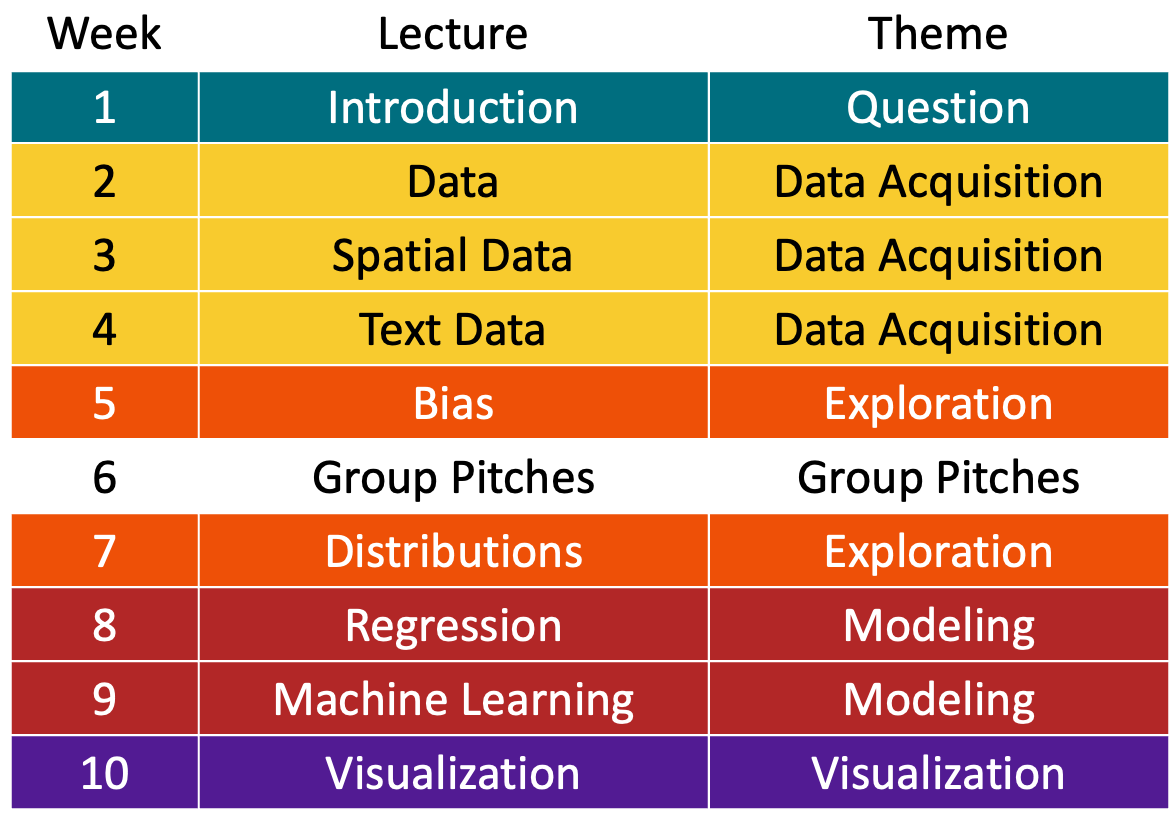
\includegraphics{outline.png}

\bookmarksetup{startatroot}

\hypertarget{python-recap}{%
\chapter{Python Recap}\label{python-recap}}

\hypertarget{workshop-1-open-in-colab}{%
\section[\emph{Workshop 1} ]{\texorpdfstring{\emph{Workshop 1}
\href{https://colab.research.google.com/github/oballinger/QM2/blob/main/notebooks/W01.\%20Python\%20Recap.ipynb}{\protect
\includegraphics{index_files/mediabag/colab-badge.png}}}{Workshop 1 Open In Colab}}\label{workshop-1-open-in-colab}}

\hypertarget{registering-a-github-account}{%
\section{Registering a GitHub
account}\label{registering-a-github-account}}

Before we get started, we need to set a few things up. GitHub is a
platform for software development and version control using Git,
allowing developers to store and manage their code. Think of it as
google docs but for code-- it will be very useful for collaborating on
your group projects later in the term, and in your future as a data
analyst.

\begin{enumerate}
\def\labelenumi{\arabic{enumi}.}
\tightlist
\item
  Use \href{https://github.com/join}{this link} to register for a GitHub
  account if you don't already have one.
\item
  Once that's done, \href{https://github.com/new}{create a new github
  repository} called ``QM2''.
\item
  In this notebook, click ``File'' and then ``Save a copy in GitHub''.
\end{enumerate}

Voila! You now have a version of this notebook saved to your own GitHub
account. \emph{You will need to do step 3 for all the workshops!} Now,
on to python.

\hypertarget{using-python}{%
\section{Using Python}\label{using-python}}

In this course, we'll make extensive use of \emph{Python}, a programming
language used widely in scientific computing and on the web. We will be
using Python as a way to manipulate, plot and analyse data. This isn't a
course about learning Python, it's about working with data - but we'll
learning a little bit of programming along the way.

By now, you should have done the prerequisites for the module, and
understand a bit about how Python is structured, what different commands
do, and so on - this is a bit of a refresher to remind you of what we
need at the beginning of term.

The particular flavour of Python we're using is \emph{iPython}, which,
as we've seen, allows us to combine text, code, images, equations and
figures in a \emph{Notebook}. This is a \emph{cell}, written in
\emph{markdown} - a way of writing nice text. Contrast this with
\emph{code} cell, which executes a bit of Python:

\begin{Shaded}
\begin{Highlighting}[]
\BuiltInTok{print}\NormalTok{(}\DecValTok{2}\OperatorTok{+}\DecValTok{2}\NormalTok{)}
\end{Highlighting}
\end{Shaded}

\begin{verbatim}
4
\end{verbatim}

The Notebook format allows you to engage in what Don Knuth describes as
\href{http://en.wikipedia.org/wiki/Literate_programming}{Literate
Programming}:

\begin{quote}
{[}\ldots{]} Instead of writing code containing documentation, the
literate programmer writes documentation containing code. No longer does
the English commentary injected into a program have to be hidden in
comment delimiters at the top of the file, or under procedure headings,
or at the end of lines. Instead, it is wrenched into the daylight and
made the main focus. The ``program'' then becomes primarily a document
directed at humans, with the code being herded between ``code
delimiters'' from where it can be extracted and shuffled out sideways to
the language system by literate programming tools.
\href{http://www.literateprogramming.com/lpquotes.html}{Ross Williams}
\end{quote}

\hypertarget{libraries}{%
\section{Libraries}\label{libraries}}

We will work with a number of \emph{libraries}, which provide additional
functions and techniques to help us to carry out our tasks.

These include:

\emph{Pandas:} we'll use this a lot to slice and dice data

\emph{matplotlib}: this is our basic graphing software, and we'll also
use it for mapping

\emph{nltk}: The Natural Language Tool Kit will help us work with text

We aren't doing all this to learn to program. We could spend a whole
term learning how to use Python and never look at any data, maps,
graphs, or visualisations. But we do need to understand a few basics to
use Python for working with data. So let's revisit a few concepts that
you should have covered in your prerequisites.

\hypertarget{variables}{%
\section{Variables}\label{variables}}

Python can broadly be divided in verbs and nouns: things which \emph{do}
things, and things which \emph{are} things. In Python, the verbs can be
\emph{commands}, \emph{functions}, or \emph{methods}. We won't worry too
much about the distinction here - suffice it to say, they are the parts
of code which manipulate data, calculate values, or show things on the
screen.

The simplest proper noun object in Python is the \emph{variable}.
Variables are given names and store information. This can be, for
example, numeric, text, or boolean (true/false). These are all
statements setting up variables:

n = 1

t = ``hi''

b = True

Now let's try this in code:

\begin{Shaded}
\begin{Highlighting}[]
\NormalTok{n }\OperatorTok{=} \DecValTok{1}

\NormalTok{t }\OperatorTok{=} \StringTok{"hi"}

\NormalTok{b }\OperatorTok{=} \VariableTok{True}
\end{Highlighting}
\end{Shaded}

Note that each command is on a new line; other than that, the
\emph{syntax} of Python should be fairly clear. We're setting these
variables equal to the letters and numbers and phrases and booleans.
\textbf{What's a boolean?}

The value of this is we now have values tied to these variables - so
every time we want to use it, we can refer to the variable:

\begin{Shaded}
\begin{Highlighting}[]
\NormalTok{n}
\end{Highlighting}
\end{Shaded}

\begin{verbatim}
1
\end{verbatim}

\begin{Shaded}
\begin{Highlighting}[]
\NormalTok{t}
\end{Highlighting}
\end{Shaded}

\begin{verbatim}
'hi'
\end{verbatim}

\begin{Shaded}
\begin{Highlighting}[]
\NormalTok{b}
\end{Highlighting}
\end{Shaded}

\begin{verbatim}
True
\end{verbatim}

Because we've defined these variables in the early part of the notebook,
we can use them later on.

\emph{\textbf{Advanced}: where do \textbf{classes} fit into this
noun/verb picture of variables and commands?}

\hypertarget{where-is-my-data}{%
\section{Where is my data?}\label{where-is-my-data}}

When we work in excel and text editors, we're used to seeing the data
onscreen - and if we manipulate the data in some way (averaging or
summing up), we see both the inputs and outputs on screen. The big
difference in working with Python is that we don't see our variables all
of the time, or the effect we're having on them. They're there in the
background, but it's usually worth checking in on them from time to
time, to see whether our processes are doing what we think they're
doing.

This is pretty easy to do - we can just type the variable name, or
``print(\emph{variable name})'':

\begin{Shaded}
\begin{Highlighting}[]
\NormalTok{n }\OperatorTok{=}\NormalTok{ n}\OperatorTok{+}\DecValTok{1}
\BuiltInTok{print}\NormalTok{(n)}
\BuiltInTok{print}\NormalTok{(t)}
\BuiltInTok{print}\NormalTok{(b)}
\end{Highlighting}
\end{Shaded}

\begin{verbatim}
2
hi
True
\end{verbatim}

\hypertarget{flow}{%
\section{Flow}\label{flow}}

Python, in common with all programming languages, executes commands in a
sequence - we might refer to this as the ``ineluctable march of the
machines'', but it's more common referred to as the \emph{flow} of the
code (we'll use the word ``code'' a lot - it just means commands written
in the programming language). In most cases, code just executes in the
order it's written. This is true within each \emph{cell} (each block of
text in the notebook), and it's true when we execute the cells in order;
that's why we can refer back to the variables we defined earlier:

\begin{Shaded}
\begin{Highlighting}[]
\BuiltInTok{print}\NormalTok{(n)}
\end{Highlighting}
\end{Shaded}

\begin{verbatim}
2
\end{verbatim}

If we make a change to one of these variables, say n:

\begin{Shaded}
\begin{Highlighting}[]
\NormalTok{n }\OperatorTok{=} \DecValTok{3}
\end{Highlighting}
\end{Shaded}

and execute the above ``print n'' command, you'll see that it has
changed n to 3. So if we go out of order, the obvious flow of the code
is confused. For this reason, try to write your code so it executes in
order, one cell at a time. At least for the moment, this will make it
easier to follow the logic of what you're doing to data.

\emph{Advanced}: what happens to this flow when you write
\emph{functions} to automate common tasks?

\textbf{\emph{Exercise - Setting up variables}}:

\begin{enumerate}
\def\labelenumi{\arabic{enumi}.}
\item
  Create a new cell.
\item
  Create the variables ``name'', and assign your name to it.
\item
  Create a variable ``Python'' and assign a score out of 10 to how much
  you like Python.
\item
  Create a variable ``prior'' and if you've used Python before, assign
  True; otherwise assign False to the variable
\item
  Print these out to the screen
\end{enumerate}

\hypertarget{downloading-data}{%
\section{Downloading Data}\label{downloading-data}}

Lets fetch the data we will be using for this session. There are two
ways in which you can upload data to the Colab notebook. You can use the
following code to upload a CSV or similar data file.

\begin{Shaded}
\begin{Highlighting}[]
\ImportTok{from}\NormalTok{ google.colab }\ImportTok{import}\NormalTok{ files}
\NormalTok{uploaded }\OperatorTok{=}\NormalTok{ files.upload()}
\end{Highlighting}
\end{Shaded}

Or you can use the following cell to fetch the data directly from the
QM2 server.

Let's create a folder that we can store all our data for this session

\begin{Shaded}
\begin{Highlighting}[]
\OperatorTok{!}\NormalTok{mkdir data}
\end{Highlighting}
\end{Shaded}

\begin{Shaded}
\begin{Highlighting}[]
\OperatorTok{!}\NormalTok{mkdir .}\OperatorTok{/}\NormalTok{data}\OperatorTok{/}\NormalTok{wk1}
\OperatorTok{!}\NormalTok{curl https:}\OperatorTok{//}\NormalTok{s3.eu}\OperatorTok{{-}}\NormalTok{west}\OperatorTok{{-}}\FloatTok{2.}\ErrorTok{amazonaws}\NormalTok{.com}\OperatorTok{/}\NormalTok{qm2}\OperatorTok{/}\NormalTok{wk1}\OperatorTok{/}\NormalTok{data.csv }\OperatorTok{{-}}\NormalTok{o .}\OperatorTok{/}\NormalTok{data}\OperatorTok{/}\NormalTok{wk1}\OperatorTok{/}\NormalTok{data.csv}
\OperatorTok{!}\NormalTok{curl https:}\OperatorTok{//}\NormalTok{s3.eu}\OperatorTok{{-}}\NormalTok{west}\OperatorTok{{-}}\FloatTok{2.}\ErrorTok{amazonaws}\NormalTok{.com}\OperatorTok{/}\NormalTok{qm2}\OperatorTok{/}\NormalTok{wk1}\OperatorTok{/}\NormalTok{sample\_group.csv }\OperatorTok{{-}}\NormalTok{o .}\OperatorTok{/}\NormalTok{data}\OperatorTok{/}\NormalTok{wk1}\OperatorTok{/}\NormalTok{sample\_group.csv}
\end{Highlighting}
\end{Shaded}

\begin{verbatim}
  % Total    % Received % Xferd  Average Speed   Time    Time     Time  Current
                                 Dload  Upload   Total   Spent    Left  Speed
100   203  100   203    0     0   2872      0 --:--:-- --:--:-- --:--:--  3029
  % Total    % Received % Xferd  Average Speed   Time    Time     Time  Current
                                 Dload  Upload   Total   Spent    Left  Speed
100   297  100   297    0     0   1844      0 --:--:-- --:--:-- --:--:--  1879
\end{verbatim}

\hypertarget{storing-and-importing-data}{%
\section{Storing and importing data}\label{storing-and-importing-data}}

Typically, data we look at won't be just one number, or one bit of text.
Python has a lot of different ways of dealing with a bunch of numbers:
for example, a list of values is called a \textbf{list}:

\begin{Shaded}
\begin{Highlighting}[]
\NormalTok{listy }\OperatorTok{=}\NormalTok{ [}\DecValTok{1}\NormalTok{,}\DecValTok{2}\NormalTok{,}\DecValTok{3}\NormalTok{,}\DecValTok{6}\NormalTok{,}\DecValTok{9}\NormalTok{]}
\BuiltInTok{print}\NormalTok{(listy)}
\end{Highlighting}
\end{Shaded}

\begin{verbatim}
[1, 2, 3, 6, 9]
\end{verbatim}

A set of values \emph{linked} to an index (or key) is called a
\textbf{dictionary}; for example:

\begin{Shaded}
\begin{Highlighting}[]
\NormalTok{dicty }\OperatorTok{=}\NormalTok{ \{}\StringTok{\textquotesingle{}Bob\textquotesingle{}}\NormalTok{: }\FloatTok{1.2}\NormalTok{, }\StringTok{\textquotesingle{}Mike\textquotesingle{}}\NormalTok{: }\FloatTok{1.2}\NormalTok{, }\StringTok{\textquotesingle{}Coop\textquotesingle{}}\NormalTok{: }\FloatTok{1.1}\NormalTok{, }\StringTok{\textquotesingle{}Maddy\textquotesingle{}}\NormalTok{: }\FloatTok{1.3}\NormalTok{, }\StringTok{\textquotesingle{}Giant\textquotesingle{}}\NormalTok{: }\FloatTok{2.1}\NormalTok{\}}
\BuiltInTok{print}\NormalTok{(dicty)}
\end{Highlighting}
\end{Shaded}

\begin{verbatim}
{'Bob': 1.2, 'Mike': 1.2, 'Coop': 1.1, 'Maddy': 1.3, 'Giant': 2.1}
\end{verbatim}

Notice that the list uses square brackets with values separated by
commas, and the dict uses curly brackets with pairs separated by commas,
and colons (:) to link a \emph{key} (index or address) with a value.

(You might notice that they haven't printed out in the order you entered
them)

*\textbf{Advanced}: Print out 1) The third element of \textbf{listy},
and 2) The element of \textbf{dicty} relating to Giant

We'll discuss different ways of organising data again soon, but for now
we'll look at \emph{dataframes} - the way our data-friendly
\emph{library} \textbf{Pandas} works with data. We'll be using Pandas a
lot this term, so it's good to get started with it early.

Let's start by importing pandas. We'll also import another library, but
we're not going to worry about that too much at the moment.

If you see a warning about `Building Font Cache' don't worry - this is
normal.

\begin{Shaded}
\begin{Highlighting}[]
\ImportTok{import}\NormalTok{ pandas}

\ImportTok{import}\NormalTok{ matplotlib}
\OperatorTok{\%}\NormalTok{matplotlib inline}
\end{Highlighting}
\end{Shaded}

Let's import a simple dataset and show it in pandas. We'll use a
pre-prepared ``.csv'' file, which needs to be in the same folder as our
code.

\begin{Shaded}
\begin{Highlighting}[]
\NormalTok{data }\OperatorTok{=}\NormalTok{ pandas.read\_csv(}\StringTok{\textquotesingle{}./data/wk1/data.csv\textquotesingle{}}\NormalTok{)}
\NormalTok{data.head()}
\end{Highlighting}
\end{Shaded}

\begin{longtable}[]{@{}llllll@{}}
\toprule\noalign{}
& Name & First Appearance & Approx height & Gender & Law Enforcement \\
\midrule\noalign{}
\endhead
\bottomrule\noalign{}
\endlastfoot
0 & Bob & 1.2 & 6.0 & Male & False \\
1 & Mike & 1.2 & 5.5 & Male & False \\
2 & Coop & 1.1 & 6.0 & Male & True \\
3 & Maddy & 1.3 & 5.5 & Female & False \\
4 & Giant & 2.1 & 7.5 & Male & False \\
\end{longtable}

What we've done here is read in a .csv file into a dataframe, the object
pandas uses to work with data, and one that has lots of methods for
slicing and dicing data, as we will see over the coming weeks. The
head() command tells iPython to show the first few columns/rows of the
data, so we can start to get a sense of what the data looks like and
what sort of type of objects is represents.

A common first step for exploring our data is to sort it. In Pandas,
this can be done easily with the \texttt{sort\_values()} function. We
can specify which column to sort the data by, and whether we want to
sort in ascending or descending order, using the optional arguments
\texttt{by} and \texttt{ascending}, respectively. In the example below,
we're sorting in \emph{descending} order of height:

\begin{Shaded}
\begin{Highlighting}[]
\NormalTok{data.sort\_values(by}\OperatorTok{=}\StringTok{\textquotesingle{}Approx height\textquotesingle{}}\NormalTok{, ascending}\OperatorTok{=}\VariableTok{False}\NormalTok{).head()}
\end{Highlighting}
\end{Shaded}

\begin{longtable}[]{@{}llllll@{}}
\toprule\noalign{}
& Name & First Appearance & Approx height & Gender & Law Enforcement \\
\midrule\noalign{}
\endhead
\bottomrule\noalign{}
\endlastfoot
4 & Giant & 2.1 & 7.5 & Male & False \\
0 & Bob & 1.2 & 6.0 & Male & False \\
2 & Coop & 1.1 & 6.0 & Male & True \\
1 & Mike & 1.2 & 5.5 & Male & False \\
3 & Maddy & 1.3 & 5.5 & Female & False \\
\end{longtable}

\bookmarksetup{startatroot}

\hypertarget{supplementary-kaggle-exercises}{%
\chapter{Supplementary: Kaggle
exercises}\label{supplementary-kaggle-exercises}}

If you've gotten this far, congratulations! To further hone your skills,
try working your way through the five
\href{https://www.kaggle.com/learn/intro-to-programming}{intro to
programming notebooks on Kaggle}. These cover a range of skills that
we'll be using throughout the term. Kaggle is a very useful resource for
learning data science, so making an account may not be a bad idea!

\bookmarksetup{startatroot}

\hypertarget{assessed-question}{%
\chapter{Assessed Question}\label{assessed-question}}

The URL below contains a dataset of the most streamed songs on spotify
in 2023: https://storage.googleapis.com/qm2/wk1/spotify-2023.csv

\begin{enumerate}
\def\labelenumi{\arabic{enumi}.}
\tightlist
\item
  Download the dataset and save it in the \texttt{./data/wk1/}
  directory.
\item
  Load the dataset as a pandas dataframe, and inspect it. Two of the
  column names have accidentally been swapped around. Use common sense
  to figure out which ones these are before proceeding with your
  analysis.
\item
  Filter the dataset to only contain songs in the key of C sharp.
\item
  Sort the dataframe in descending order of streams.
\end{enumerate}

QUESTION: which artist has the highest number of streams?

\begin{Shaded}
\begin{Highlighting}[]
\CommentTok{\# use this code cell to answer the question}
\end{Highlighting}
\end{Shaded}

\bookmarksetup{startatroot}

\hypertarget{intro-to-pandas}{%
\chapter{Intro to Pandas}\label{intro-to-pandas}}

\hypertarget{workshop-2-open-in-colab}{%
\section[\emph{Workshop 2} ]{\texorpdfstring{\emph{Workshop 2}
\href{https://colab.research.google.com/github/oballinger/QM2/blob/main/notebooks/W02.\%20Pandas.ipynb}{\protect
\includegraphics{notebooks/../colab-badge.png}}}{Workshop 2 Open In Colab}}\label{workshop-2-open-in-colab}}

In this workshop, our aim is to get used to working with more complex
data that we've imported from external files. We'll start to graph it,
and to slice and dice it, to select the bits we're interested in.

We will work with \emph{pandas} to manipulate the data, and to derive
measures and graphs that tell us a bit more than what the source data
files tell us.

\hypertarget{aims}{%
\subsection{Aims}\label{aims}}

\begin{itemize}
\tightlist
\item
  Learn to import data to python using pandas
\item
  Learn how access specific rows, columns and cells
\item
  Plot the data
\item
  Tidy up graphs to include axes
\end{itemize}

\hypertarget{introduction}{%
\section{Introduction}\label{introduction}}

We are going to work with some UK income data. The income data is
packaged as a .csv file. The Pandas package knows how to handle this and
put the data in a DataFrame, as we've seen. Let's examine the data and
start to see what we can say about it. First of all, we have to find
data - I'm interested in looking in data with a wide spread, so I looked
for data on income in the UK.

This data is collected by the Office for National Statistics(ONS) :
http://www.ons.gov.uk/ons/datasets-and-tables/index.html?pageSize=50\&sortBy=none\&sortDirection=none\&newquery=income+percentile
- but the exact data I want to see, income by percentile, is tricky to
find.

I ended up using data from 2011, generated from a study called the
Family Resources Survey and collated and tweaked by an independent
research unit called the Institute of Fiscal Studies (IFS). The
``tweaking'' they do tends to be around the size of the family unit, and
other factors which create economies of scale - hence they
``equivalise'' it. The IFS is quoted in UK Government documents, so we
can have some trust in their impartiality, or at least accuracy - of
course, if we were publishing research about this, that's not really
good enough and we'd want to reproduce, or at least understand and
critique, their methodology rather than just trusting it!

e.g.:

http://www.ifs.org.uk/wheredoyoufitin/about.php

https://en.wikipedia.org/wiki/Equivalisation

\hypertarget{downloading-the-data}{%
\section{Downloading the Data}\label{downloading-the-data}}

Let's grab our income data from our course website and save it into our
data folder. If you've not already created a data folder then do so
using the following command. Don't worry if it generates an error, that
means you've already got a data folder.

\begin{Shaded}
\begin{Highlighting}[]
\OperatorTok{!}\NormalTok{mkdir data}
\end{Highlighting}
\end{Shaded}

\begin{verbatim}
mkdir: data: File exists
\end{verbatim}

\begin{Shaded}
\begin{Highlighting}[]
\OperatorTok{!}\NormalTok{mkdir data}\OperatorTok{/}\NormalTok{wk2}
\OperatorTok{!}\NormalTok{curl https:}\OperatorTok{//}\NormalTok{s3.eu}\OperatorTok{{-}}\NormalTok{west}\OperatorTok{{-}}\FloatTok{2.}\ErrorTok{amazonaws}\NormalTok{.com}\OperatorTok{/}\NormalTok{qm2}\OperatorTok{/}\NormalTok{wk2}\OperatorTok{/}\NormalTok{incomes.csv }\OperatorTok{{-}}\NormalTok{o .}\OperatorTok{/}\NormalTok{data}\OperatorTok{/}\NormalTok{wk2}\OperatorTok{/}\NormalTok{incomes.csv}
\end{Highlighting}
\end{Shaded}

\begin{verbatim}
mkdir: data/wk2: File exists
  % Total    % Received % Xferd  Average Speed   Time    Time     Time  Current
                                 Dload  Upload   Total   Spent    Left  Speed
100 15154  100 15154    0     0   135k      0 --:--:-- --:--:-- --:--:--  143k
\end{verbatim}

\begin{Shaded}
\begin{Highlighting}[]
\ImportTok{import}\NormalTok{ pandas}
\ImportTok{import}\NormalTok{ pylab}
\ImportTok{import}\NormalTok{ matplotlib.pyplot }\ImportTok{as}\NormalTok{ plt}
\CommentTok{\# make the plots a little wider by default}
\OperatorTok{\%}\NormalTok{matplotlib inline}
\NormalTok{plt.style.use(}\StringTok{\textquotesingle{}ggplot\textquotesingle{}}\NormalTok{)}

\NormalTok{pylab.rcParams[}\StringTok{\textquotesingle{}figure.figsize\textquotesingle{}}\NormalTok{] }\OperatorTok{=}\NormalTok{ (}\FloatTok{10.}\NormalTok{, }\FloatTok{8.}\NormalTok{)}
\end{Highlighting}
\end{Shaded}

\begin{Shaded}
\begin{Highlighting}[]
\NormalTok{data\_path }\OperatorTok{=} \StringTok{"./data/wk2/incomes.csv"}

\NormalTok{income }\OperatorTok{=}\NormalTok{  pandas.read\_csv(data\_path, index\_col}\OperatorTok{=}\DecValTok{0}\NormalTok{)}
\NormalTok{income.head()}
\end{Highlighting}
\end{Shaded}

\begin{longtable}[]{@{}llllllllllllllll@{}}
\toprule\noalign{}
& Net equivalised household income in 2010-11, week & Childless couple,
annual income & Couple, two children under 14 & Couple, three children
under 14 & Couple with one child under 14 & Couple with two children
aged 15 to 18 & Couple, two children under 14 plus dependent adult &
Single adult & Lone parent, one child under 14 & Lone parent, two
children under 14 & Lone parent, two children aged 15-18 & ANNOTATIONS &
1979 to 1996-97 & 1996-97 to 2009-10 & 1996-97 to 2010-11 \\
Percentile Point & & & & & & & & & & & & & & & \\
\midrule\noalign{}
\endhead
\bottomrule\noalign{}
\endlastfoot
1 & 33.50 & 1,746.92 & 2,445.69 & 2,795.08 & 2,096.31 & 2,899.89 &
3,022.18 & 1,170.44 & 1,519.82 & 1,869.21 & 2,323.41 & NaN & NaN & NaN &
NaN \\
2 & 98.60 & 5,141.01 & 7,197.41 & 8,225.61 & 6,169.21 & 8,534.07 &
8,893.95 & 3,444.48 & 4,472.68 & 5,500.88 & 6,837.54 & NaN & -0.20\% &
-1.30\% & -0.50\% \\
3 & 128.56 & 6,703.11 & 9,384.36 & 10,724.98 & 8,043.74 & 11,127.17 &
11,596.39 & 4,491.09 & 5,831.71 & 7,172.33 & 8,915.14 & NaN & 0.40\% &
0.10\% & 0.10\% \\
4 & 151.05 & 7,875.75 & 11,026.05 & 12,601.20 & 9,450.90 & 13,073.75 &
13,625.05 & 5,276.75 & 6,851.90 & 8,427.05 & 10,474.75 & NaN & 0.50\% &
0.80\% & 0.60\% \\
5 & 166.32 & 8,671.91 & 12,140.68 & 13,875.06 & 10,406.30 & 14,395.38 &
15,002.41 & 5,810.18 & 7,544.57 & 9,278.95 & 11,533.65 & NaN & 0.70\% &
1.00\% & 0.90\% \\
\end{longtable}

This is a simple dataframe - we see the percentile and an income. Note
that I've told pandas to use the first column (the Percentile) as the
index to make life easier.

The percentile tells us how people on that income rank - so the final
category, 99\% (which is really binned, so 99\%\textless n\(\leq\)
100\%), is telling us how much ``the 1\%'' earn. Let's find out:

\begin{Shaded}
\begin{Highlighting}[]
\NormalTok{income.tail()}
\end{Highlighting}
\end{Shaded}

\begin{longtable}[]{@{}llllllllllllllll@{}}
\toprule\noalign{}
& Net equivalised household income in 2010-11, week & Childless couple,
annual income & Couple, two children under 14 & Couple, three children
under 14 & Couple with one child under 14 & Couple with two children
aged 15 to 18 & Couple, two children under 14 plus dependent adult &
Single adult & Lone parent, one child under 14 & Lone parent, two
children under 14 & Lone parent, two children aged 15-18 & ANNOTATIONS &
1979 to 1996-97 & 1996-97 to 2009-10 & 1996-97 to 2010-11 \\
Percentile Point & & & & & & & & & & & & & & & \\
\midrule\noalign{}
\endhead
\bottomrule\noalign{}
\endlastfoot
95 & 1075.73 & 56,088.56 & 78,523.99 & 89,741.70 & 67,306.27 & 93,107.01
& 97,033.21 & 37,579.34 & 48,797.05 & 60,014.76 & 74,597.79 & NaN &
2.90\% & 2.00\% & 1.30\% \\
96 & 1174.48 & 61,237.18 & 85,732.05 & 97,979.49 & 73,484.61 &
101,653.72 & 105,940.32 & 41,028.91 & 53,276.35 & 65,523.78 & 81,445.45
& NaN & 3.00\% & 2.00\% & 1.40\% \\
97 & 1302.74 & 67,925.07 & 95,095.10 & 108,680.12 & 81,510.09 &
112,755.62 & 117,510.37 & 45,509.80 & 59,094.81 & 72,679.83 & 90,340.35
& NaN & 3.20\% & 2.20\% & 1.60\% \\
98 & 1523.31 & 79,425.23 & 111,195.32 & 127,080.36 & 95,310.27 &
131,845.88 & 137,405.64 & 53,214.90 & 69,099.95 & 84,984.99 & 105,635.55
& NaN & 3.20\% & 2.70\% & 1.70\% \\
99 & 2090.35 & 108,990.74 & 152,587.04 & 174,385.19 & 130,788.89 &
180,924.64 & 188,553.99 & 73,023.80 & 94,821.95 & 116,620.10 &
144,957.69 & NaN & NaN & NaN & NaN \\
\end{longtable}

Well, they we have it - the 1\% earn, on average, about £2000 a week.
How does that compare to people in the 90\% decile? We can access
particular \emph{rows} in a dataframe using \textbf{.loc{[}row
index{]}}; because our index is the percentile point, we can just read
it off:

\begin{Shaded}
\begin{Highlighting}[]
\NormalTok{income.loc[}\DecValTok{90}\NormalTok{]}
\end{Highlighting}
\end{Shaded}

\begin{verbatim}
Net equivalised household income in 2010-11, week        845.54
Childless couple, annual income                       44,086.54
Couple, two children under 14                         61,721.15
Couple, three children under 14                       70,538.46
Couple with one child under 14                        52,903.85
Couple with two children aged 15 to 18                73,183.65
Couple, two children under 14 plus dependent adult    76,269.71
Single adult                                          29,537.98
Lone parent, one child under 14                       38,355.29
Lone parent, two children under 14                    47,172.60
Lone parent, two children aged 15-18                  58,635.10
ANNOTATIONS                                                 NaN
1979 to 1996-97                                           2.50%
1996-97 to 2009-10                                        1.70%
1996-97 to 2010-11                                        1.20%
Name: 90, dtype: object
\end{verbatim}

We can also select a range of values with the ``colon'' notation. This
will select the 90-95th percentiles, for example:

\begin{Shaded}
\begin{Highlighting}[]
\NormalTok{income.loc[}\DecValTok{90}\NormalTok{:}\DecValTok{95}\NormalTok{]}
\end{Highlighting}
\end{Shaded}

\begin{longtable}[]{@{}llllllllllllllll@{}}
\toprule\noalign{}
& Net equivalised household income in 2010-11, week & Childless couple,
annual income & Couple, two children under 14 & Couple, three children
under 14 & Couple with one child under 14 & Couple with two children
aged 15 to 18 & Couple, two children under 14 plus dependent adult &
Single adult & Lone parent, one child under 14 & Lone parent, two
children under 14 & Lone parent, two children aged 15-18 & ANNOTATIONS &
1979 to 1996-97 & 1996-97 to 2009-10 & 1996-97 to 2010-11 \\
Percentile Point & & & & & & & & & & & & & & & \\
\midrule\noalign{}
\endhead
\bottomrule\noalign{}
\endlastfoot
90 & 845.54 & 44,086.54 & 61,721.15 & 70,538.46 & 52,903.85 & 73,183.65
& 76,269.71 & 29,537.98 & 38,355.29 & 47,172.60 & 58,635.10 & NaN &
2.50\% & 1.70\% & 1.20\% \\
91 & 876.63 & 45,707.74 & 63,990.84 & 73,132.39 & 54,849.29 & 75,874.85
& 79,074.40 & 30,624.19 & 39,765.74 & 48,907.29 & 60,791.30 & NaN &
2.60\% & 1.70\% & 1.20\% \\
92 & 911.29 & 47,514.54 & 66,520.35 & 76,023.26 & 57,017.44 & 78,874.13
& 82,200.15 & 31,834.74 & 41,337.65 & 50,840.55 & 63,194.33 & NaN &
2.60\% & 1.80\% & 1.20\% \\
93 & 957.14 & 49,905.23 & 69,867.32 & 79,848.36 & 59,886.27 & 82,842.68
& 86,336.04 & 33,436.50 & 43,417.55 & 53,398.59 & 66,373.95 & NaN &
2.70\% & 1.80\% & 1.30\% \\
94 & 1016.37 & 52,993.38 & 74,190.73 & 84,789.40 & 63,592.05 & 87,969.00
& 91,678.54 & 35,505.56 & 46,104.24 & 56,702.91 & 70,481.19 & NaN &
2.90\% & 1.90\% & 1.30\% \\
95 & 1075.73 & 56,088.56 & 78,523.99 & 89,741.70 & 67,306.27 & 93,107.01
& 97,033.21 & 37,579.34 & 48,797.05 & 60,014.76 & 74,597.79 & NaN &
2.90\% & 2.00\% & 1.30\% \\
\end{longtable}

\hypertarget{accessing-parts-of-a-dataframe}{%
\section{Accessing parts of a
dataframe}\label{accessing-parts-of-a-dataframe}}

If we want to extract the actual value instead of just the whole row, we
need to reference the \emph{column} as well as the row. In pandas,
columns are referenced by \textbf{column name}:

\begin{Shaded}
\begin{Highlighting}[]
\NormalTok{income[}\StringTok{\textquotesingle{}Net equivalised household income in 2010{-}11, week\textquotesingle{}}\NormalTok{]}
\end{Highlighting}
\end{Shaded}

\begin{verbatim}
Percentile Point
1       33.50
2       98.60
3      128.56
4      151.05
5      166.32
       ...   
95    1075.73
96    1174.48
97    1302.74
98    1523.31
99    2090.35
Name: Net equivalised household income in 2010-11, week, Length: 99, dtype: float64
\end{verbatim}

So, to access a particular cell, we tell Python the row and the column
(this is pretty simple - the same way we tell excel to access cell
``A34'' meaning Column A, Row 34). One way we do that in pandas is to
select the column, and then use .loc{[}{]} on the index.

\begin{Shaded}
\begin{Highlighting}[]
\NormalTok{income[}\StringTok{\textquotesingle{}Net equivalised household income in 2010{-}11, week\textquotesingle{}}\NormalTok{].loc[}\DecValTok{90}\NormalTok{]}
\end{Highlighting}
\end{Shaded}

\begin{verbatim}
845.54
\end{verbatim}

We've accessed row 90 of the column called `Net equivalised household
income in 2010-11, week'; can we access the data the other way around -
can we first take the row and then specify a column? Let's try:

\begin{Shaded}
\begin{Highlighting}[]
\NormalTok{income.loc[}\DecValTok{90}\NormalTok{][}\StringTok{\textquotesingle{}Net equivalised household income in 2010{-}11, week\textquotesingle{}}\NormalTok{]}
\end{Highlighting}
\end{Shaded}

\begin{verbatim}
845.54
\end{verbatim}

Yes, this seems to be working fine.

\hypertarget{extension}{%
\subsection{Extension}\label{extension}}

The reason for this is that selecting the column spits out a smaller
dataframe, and all dataframes use ``loc'', so we can use that. Another
way to do this would be to use an explicit variable for the dataframe,
along the lines of:

\texttt{smallDataFrame\ =\ income{[}\textquotesingle{}Net\ equivalised\ household\ income\ in\ 2010-11,\ week\textquotesingle{}{]}}\strut \\
\texttt{smallDataFrame.loc{[}90{]}}

by doing income

\texttt{{[}\textquotesingle{}Net\ equivalised\ household\ income\ in\ 2010-11,\ week\textquotesingle{}{]}.loc{[}90{]}}

we're taking the ``smallDataFrame'' object as an implicit (or hidden)
output

If we want to look at a few rows of data, we can use a range:

\begin{Shaded}
\begin{Highlighting}[]
\NormalTok{income[}\StringTok{\textquotesingle{}Net equivalised household income in 2010{-}11, week\textquotesingle{}}\NormalTok{].loc[}\DecValTok{90}\NormalTok{:}\DecValTok{95}\NormalTok{]}
\end{Highlighting}
\end{Shaded}

\begin{verbatim}
Percentile Point
90     845.54
91     876.63
92     911.29
93     957.14
94    1016.37
95    1075.73
Name: Net equivalised household income in 2010-11, week, dtype: float64
\end{verbatim}

So, to recap, we can now access a particular \textbf{row} using
\emph{loc{[}index number{]}}, a particular \textbf{column} with the
square brackets formalism \emph{dataframename{[}`column name'{]}}, or
both \emph{dataframename{[}`column name'{]}.loc{[}index number{]}}.
We've made a start at being able to get to the bits of data we need.

\hypertarget{exercise}{%
\section{Exercise:}\label{exercise}}

How do the equivalised incomes of single adults and childless couples
compare? Look at the 1st, 99th and 50th percentile and summarise what
this tells you about the value or price of coupling.

\hypertarget{examining-the-distribution}{%
\section{Examining the Distribution}\label{examining-the-distribution}}

Returning to the overall statistics, the 90\% percentile earns less than
half the top percentile (``the 1\%''); if you're taking home over £800
as a household, you're in the top 10\% of earners.

How does 1. The income of ``the 1\%'' compare with the mean and median
across the population, as a proportion? 2. How does the 1\% compare with
the 90th percentile (the 10\%)? 3. How does the 10\% compare with the
median and mean?

The 1\% earn about 60 times the poorest groups in society - and we've
made other comparisons. But that's not the whole story. Let's look at
the income graph.

In pandas, we can plot this fairly easily\ldots{}

\begin{Shaded}
\begin{Highlighting}[]
\NormalTok{income[}\StringTok{\textquotesingle{}Net equivalised household income in 2010{-}11, week\textquotesingle{}}\NormalTok{].plot()}
\NormalTok{plt.title(}\StringTok{\textquotesingle{}UK Net Equivalised Income by Percentile per week, 2010{-}11\textquotesingle{}}\NormalTok{)}
\NormalTok{plt.xlabel(}\StringTok{\textquotesingle{}Income Percentile\textquotesingle{}}\NormalTok{)}
\NormalTok{plt.ylabel(}\StringTok{\textquotesingle{}Income (Net, Equivalised) [GBP]\textquotesingle{}}\NormalTok{)}
\end{Highlighting}
\end{Shaded}

\begin{verbatim}
Text(0, 0.5, 'Income (Net, Equivalised) [GBP]')
\end{verbatim}

\begin{figure}[H]

{\centering 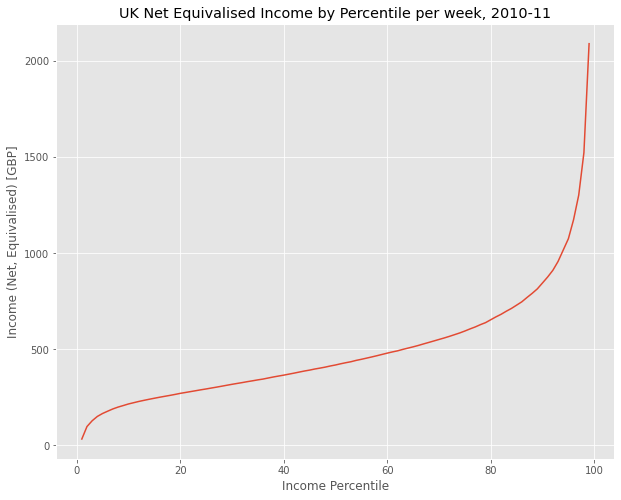
\includegraphics{notebooks/W02. Pandas_files/figure-pdf/cell-13-output-2.png}

}

\end{figure}

We see a curve that is pretty linear in the middle region, but curves
rapidly upwards in the higher percentile and looks more like a power
law.

\hypertarget{exercise-means}{%
\subsection{Exercise: Means}\label{exercise-means}}

Where does the mean appear here? Draw in a horizontal line to show the
mean using \textbf{axhline}. Show the median on the same graph. What is
the meaning of the median in this context?

Hint: Recall that last time we used \emph{axvline} to highlight the mean
and standard deviation by drawing vertical lines on the axis. Here, we
use \emph{axhline} to draw horizontal lines.

\hypertarget{extension-accessing-cells}{%
\subsection{Extension: Accessing
cells}\label{extension-accessing-cells}}

There are a number of ways to access elements of the dataframe: we've
shown how to access columns by the {[}\emph{`name of column'}{]} method,
and rows via the .loc{[}\emph{index}{]} method; and how we can select a
range. There are also .iloc methods to select by number rather than
name; you should become familiar with these on the documentation page
for pandas.

\hypertarget{comparing-segments}{%
\section{Comparing segments}\label{comparing-segments}}

Earlier, we compared some summary statistics of single people and
couples. Let's look at the wider curve for more than one group, now:

\begin{Shaded}
\begin{Highlighting}[]
\CommentTok{\#This is going to throw a load of errors}
\NormalTok{income[[}\StringTok{\textquotesingle{}Single adult\textquotesingle{}}\NormalTok{,}\StringTok{\textquotesingle{}Lone parent, one child under 14\textquotesingle{}}\NormalTok{]].plot()}
\end{Highlighting}
\end{Shaded}

\begin{verbatim}
TypeError: no numeric data to plot
\end{verbatim}

\hypertarget{warning}{%
\section{Warning}\label{warning}}

This isn't looking good. There's a load of text and no graph. If you've
not seen this before, it's an error - something has gone wrong.
Generally, if we look at the \textbf{final} line, it should tell us
what's wrong, in this case there's ``no numeric data to plot'', which is
weird, because we've seen the data and have even plotted some of it.

\hypertarget{messy-data}{%
\section{Messy Data}\label{messy-data}}

DataFrames, as we are starting to see, give us the chance to plot, chop,
slice and data to help us make sense of it. Here, we will create a
\textbf{new} DataFrame to take only two columns of data, and get rid of
any blank cells and any cells which are not being read as numbers -
normally a sign of a missing value or a non-numerical character. Why
could this be happening? It could be

\begin{itemize}
\item
  due to blank spaces in the text file
\item
  due to letters where there should be numbers
\item
  due to characters (``,'', ``-'', etc) that shouldn't really be there
\end{itemize}

In general, there will be some detective work required to figure out
what's wrong in our text file. Your best bet is sometimes to open up the
data in a text editor, like I've done here:

\begin{Shaded}
\begin{Highlighting}[]
\ImportTok{from}\NormalTok{ IPython.display }\ImportTok{import}\NormalTok{ Image}

\NormalTok{data\_path }\OperatorTok{=} \StringTok{"https://s3.eu{-}west{-}2.amazonaws.com/qm2/wk2/data.png"}
\NormalTok{Image(data\_path)}
\end{Highlighting}
\end{Shaded}

\begin{figure}[H]

{\centering 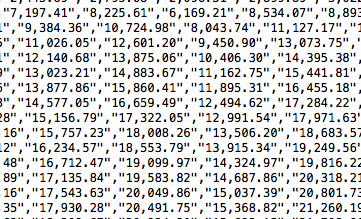
\includegraphics{notebooks/W02. Pandas_files/figure-pdf/cell-15-output-1.png}

}

\end{figure}

That's a screenshot of our datafile, opened up in a text editor. As we
can see, these numbers are separated by commas and surrounded by
quotation marks - this is normal, and what .csv files are supposed to
look like. However, there are a lot of commas within the numbers - which
makes it easier for people to read, but confuses software. Luckily,
Python has a method for dealing with this - the ``replace'' method.

Unfortunately, this dataframe is quite messy, so I'm going to have to
extract just the columns of data I'm interested in to make it work. I'll
do that by creating a new dataframe:

\hypertarget{example-cleaning-data}{%
\section{Example: Cleaning data}\label{example-cleaning-data}}

\begin{Shaded}
\begin{Highlighting}[]
\NormalTok{clean }\OperatorTok{=}\NormalTok{ income[[}\StringTok{\textquotesingle{}Childless couple, annual income\textquotesingle{}}\NormalTok{,}\StringTok{\textquotesingle{}Couple, two children under 14\textquotesingle{}}\NormalTok{]]}
\NormalTok{clean.head()}
\end{Highlighting}
\end{Shaded}

\begin{longtable}[]{@{}lll@{}}
\toprule\noalign{}
& Childless couple, annual income & Couple, two children under 14 \\
Percentile Point & & \\
\midrule\noalign{}
\endhead
\bottomrule\noalign{}
\endlastfoot
1 & 1,746.92 & 2,445.69 \\
2 & 5,141.01 & 7,197.41 \\
3 & 6,703.11 & 9,384.36 \\
4 & 7,875.75 & 11,026.05 \\
5 & 8,671.91 & 12,140.68 \\
\end{longtable}

We see those pesky commas. Now we can get on with cleaning up the data:

\begin{Shaded}
\begin{Highlighting}[]
\NormalTok{clean}\OperatorTok{=}\NormalTok{clean.replace(}\StringTok{\textquotesingle{},\textquotesingle{}}\NormalTok{, }\StringTok{\textquotesingle{}\textquotesingle{}}\NormalTok{, regex}\OperatorTok{=}\VariableTok{True}\NormalTok{)}

\CommentTok{\# In addition, missing values are sometimes written as \textquotesingle{}{-}\textquotesingle{}, in order for Python to understand that it is just a missing numerical }
\CommentTok{\# value, all \textquotesingle{}{-}\textquotesingle{} need to be replaced with \textquotesingle{}NaN\textquotesingle{}.}
\NormalTok{clean }\OperatorTok{=}\NormalTok{ clean.replace(}\StringTok{\textquotesingle{}{-}\textquotesingle{}}\NormalTok{, }\StringTok{\textquotesingle{}NaN\textquotesingle{}}\NormalTok{, regex}\OperatorTok{=}\VariableTok{True}\NormalTok{).astype(}\StringTok{\textquotesingle{}float\textquotesingle{}}\NormalTok{)}
\NormalTok{clean.head()}
\end{Highlighting}
\end{Shaded}

\begin{longtable}[]{@{}lll@{}}
\toprule\noalign{}
& Childless couple, annual income & Couple, two children under 14 \\
Percentile Point & & \\
\midrule\noalign{}
\endhead
\bottomrule\noalign{}
\endlastfoot
1 & 1746.92 & 2445.69 \\
2 & 5141.01 & 7197.41 \\
3 & 6703.11 & 9384.36 \\
4 & 7875.75 & 11026.05 \\
5 & 8671.91 & 12140.68 \\
\end{longtable}

\textbf{Extension}: ``\textbf{Regex}'' refers to ``\textbf{Reg}ular
\textbf{Ex}pression'', which is a way of replacing and cleaning text.
It's a bit beyond the scope of this class, but worth looking into if
you're interested in programming more widely.

This seems to have done the job. We've also put a line in the code to
get rid of dashes - a way that data collectors will sometimes represent
missing data. Now let's plot this.

\hypertarget{asking-more-questions-of-the-data}{%
\section{Asking more questions of the
data}\label{asking-more-questions-of-the-data}}

For me, this data starts to beg further questions. How would we answer
these?

\begin{itemize}
\item
  If the top 20\% of income shows such a sharp increase, how do we know
  that there isn't a similar uptick \emph{within} the 1\%? We've already
  seen that the mean of the dataset as a whole is much less than the
  half the maximum category (it's 25\% of the maximum). What if that's
  true within the 1\%, and £2,000/week as a fraction of the 0.1\%, or
  the 0.01\%?
\item
  How does this break down for gender, or educational background, or
  other factors like ethnicity or country of origin?
\item
  Which parts of the income curve show greater gaps between these
  subgroups and what might it say about the underlying causal
  mechanisms?
\end{itemize}

\begin{Shaded}
\begin{Highlighting}[]
\NormalTok{clean.plot()}
\NormalTok{plt.title(}\StringTok{\textquotesingle{}A Modest Proposal: The fiscal benefits of childbirth\textquotesingle{}}\NormalTok{)}
\NormalTok{plt.xlabel(}\StringTok{\textquotesingle{}Percentile\textquotesingle{}}\NormalTok{)}
\NormalTok{plt.ylabel(}\StringTok{\textquotesingle{}Income Per Week [GBP]\textquotesingle{}}\NormalTok{)}
\end{Highlighting}
\end{Shaded}

\begin{verbatim}
Text(0, 0.5, 'Income Per Week [GBP]')
\end{verbatim}

\begin{figure}[H]

{\centering 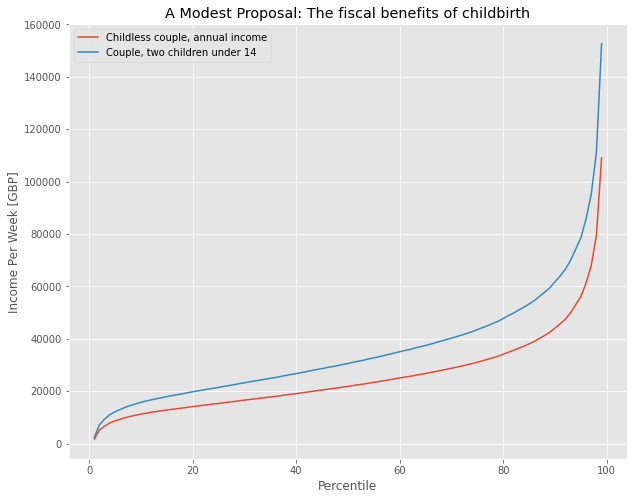
\includegraphics{notebooks/W02. Pandas_files/figure-pdf/cell-18-output-2.png}

}

\end{figure}

\hypertarget{exercise-1}{%
\section{Exercise:}\label{exercise-1}}

Previously, we'd examined income gaps between single people and couples
(how very romantic). Repeat the above exercise (cleaning and plotting
income data) for the columns we used above for single people and
childless couples. Reflect and comment on the differences.

\begin{Shaded}
\begin{Highlighting}[]
\BuiltInTok{print}\NormalTok{(}\StringTok{"Enter your code here"}\NormalTok{)}
\end{Highlighting}
\end{Shaded}

\begin{Shaded}
\begin{Highlighting}[]
\NormalTok{Add your reflection here.}
\end{Highlighting}
\end{Shaded}

So far, we've dealt with selecting data in a particular row of column by
index or label. What if we now want to filter the data by \emph{value}?
For example, let's say I want to see the data for all Childless couples
who earn more than 50,000 (net equivalised) pounds every year. This
looks like:

\begin{Shaded}
\begin{Highlighting}[]
\NormalTok{clean }\OperatorTok{=}\NormalTok{ income[[}\StringTok{\textquotesingle{}Childless couple, annual income\textquotesingle{}}\NormalTok{,}\StringTok{\textquotesingle{}Couple, two children under 14\textquotesingle{}}\NormalTok{]]}
\NormalTok{clean }\OperatorTok{=}\NormalTok{ clean.replace(}\StringTok{\textquotesingle{},\textquotesingle{}}\NormalTok{, }\StringTok{\textquotesingle{}\textquotesingle{}}\NormalTok{, regex}\OperatorTok{=}\VariableTok{True}\NormalTok{)}
\NormalTok{clean }\OperatorTok{=}\NormalTok{ clean.replace(}\StringTok{\textquotesingle{}{-}\textquotesingle{}}\NormalTok{, }\StringTok{\textquotesingle{}NaN\textquotesingle{}}\NormalTok{, regex}\OperatorTok{=}\VariableTok{True}\NormalTok{).astype(}\StringTok{\textquotesingle{}float\textquotesingle{}}\NormalTok{)}
\NormalTok{clean[clean[}\StringTok{\textquotesingle{}Childless couple, annual income\textquotesingle{}}\NormalTok{]}\OperatorTok{\textgreater{}}\DecValTok{50000}\NormalTok{]}
\end{Highlighting}
\end{Shaded}

The key line of code for selection is:

\begin{Shaded}
\begin{Highlighting}[]
\NormalTok{clean[clean[}\StringTok{\textquotesingle{}Childless couple, annual income\textquotesingle{}}\NormalTok{]}\OperatorTok{\textgreater{}}\DecValTok{50000}\NormalTok{]}
\end{Highlighting}
\end{Shaded}

Let's break this down: we're used to using \emph{dataframe}{[}\emph{some
selection}{]} from earlier. Here ``some selection'' is

\begin{Shaded}
\begin{Highlighting}[]
\NormalTok{clean[}\StringTok{\textquotesingle{}Childless couple, annual income\textquotesingle{}}\NormalTok{]}\OperatorTok{\textgreater{}}\DecValTok{50000}
\end{Highlighting}
\end{Shaded}

In other words, this command is returning a set of indices where that
statement is true. We can see this explicitly:

\begin{Shaded}
\begin{Highlighting}[]
\NormalTok{clean[}\StringTok{\textquotesingle{}Childless couple, annual income\textquotesingle{}}\NormalTok{]}\OperatorTok{\textgreater{}}\DecValTok{50000}
\end{Highlighting}
\end{Shaded}

So python is picking the values where this statement is true -
i.e.~where the `Childless couple\ldots{}' column has values greater than
50000. Then this selection is passed to the dataframe, and the dataframe
shows the correct rows.

We won't dwell on comparative operative, here we've used
``\textgreater{}'' to mean ``is greater than''; you can also use:

\begin{itemize}
\tightlist
\item
  == to mean `is equal to' {[}why the double equals?{]}
\item
  \textless\textgreater{} or != to mean `is not equal to'
\item
  \textless{} to mean `is less than'
\item
  the symbol \textgreater= to mean `is greater than or equal to'
\item
  \textless= to mean `is less than or equal to'
\end{itemize}

\hypertarget{exercise-2}{%
\section{Exercise}\label{exercise-2}}

On an approporiately labelled graph, plot the incomes of all single
adults whose net equivalised income is less than or equal to £10,000.
What proportion of the population is this?

\bookmarksetup{startatroot}

\hypertarget{extension-web-scraping}{%
\chapter{Extension: Web Scraping}\label{extension-web-scraping}}

In this example, we've been working with a .csv file that contains all
the data we want. That's not always the case. Let's say we're interested
in getting the data from a table on a website. Websites are built using
HTML code, so what we need to figure out how to look inside the
website's code and pull out the data we want. Luckily, pandas has a
built in function that can automatically recognize HTML tables in
websites and turn them into dataframes.

Let's start with the \href{https://top10.netflix.com/}{Netflix Top 10}
website. Click on the link and have a look around. You'll notice two
tables: the first showing the top 10 films this week, and the second
(farther down) showing the most popular filsms based on their first 28
days on netflix.

We can download both of these tables into python using one pandas
function: read\_html

\begin{Shaded}
\begin{Highlighting}[]
\NormalTok{url}\OperatorTok{=}\StringTok{\textquotesingle{}https://top10.netflix.com/\textquotesingle{}}

\NormalTok{tables}\OperatorTok{=}\NormalTok{pandas.read\_html(url)}

\BuiltInTok{print}\NormalTok{(tables)}
\end{Highlighting}
\end{Shaded}

\begin{verbatim}
[    #  \
0   1   
1   2   
2   3   
3   4   
4   5   
5   6   
6   7   
7   8   
8   9   
9  10   

  .css-ld8rqy-container{position:relative;box-sizing:border-box;min-width:0;}.css-7pg0cj-a11yText{z-index:9999;border:0;clip:rect(1px, 1px, 1px, 1px);height:1px;width:1px;position:absolute;overflow:hidden;padding:0;white-space:nowrap;}.css-3zcu7z-control{-webkit-align-items:center;-webkit-box-align:center;-ms-flex-align:center;align-items:center;background-color:hsl(0, 0%, 100%);border-color:hsl(0, 0%, 80%);border-radius:0;border-style:solid;border-width:1px;box-shadow:none;cursor:pointer;display:-webkit-box;display:-webkit-flex;display:-ms-flexbox;display:flex;-webkit-box-flex-wrap:wrap;-webkit-flex-wrap:wrap;-ms-flex-wrap:wrap;flex-wrap:wrap;-webkit-box-pack:justify;-webkit-justify-content:space-between;justify-content:space-between;min-height:0rem;outline:0!important;position:relative;-webkit-transition:all 100ms;transition:all 100ms;box-sizing:border-box;background:transparent;border:none;padding:0px 3px;margin-left:-5px;}.css-3zcu7z-control:hover{border-color:rgba(255,255,255,0.9);}.css-zl2g27{-webkit-align-items:center;-webkit-box-align:center;-ms-flex-align:center;align-items:center;display:grid;-webkit-flex:1;-ms-flex:1;flex:1;-webkit-box-flex-wrap:wrap;-webkit-flex-wrap:wrap;-ms-flex-wrap:wrap;flex-wrap:wrap;padding:0;-webkit-overflow-scrolling:touch;position:relative;overflow:hidden;box-sizing:border-box;}.css-hlu0h4-singleValue{color:white;grid-area:1/1/2/3;margin-left:2px;margin-right:2px;max-width:100%;overflow:hidden;text-overflow:ellipsis;white-space:nowrap;box-sizing:border-box;}Films (English).css-1a9ai41{margin:0;padding-bottom:2px;padding-top:2px;visibility:visible;color:hsl(0, 0%, 20%);-webkit-flex:1 1 auto;-ms-flex:1 1 auto;flex:1 1 auto;display:inline-grid;grid-area:1/1/2/3;grid-template-columns:0 min-content;box-sizing:border-box;padding:0;}.css-1a9ai41:after{content:attr(data-value) " ";visibility:hidden;white-space:pre;grid-area:1/2;font:inherit;min-width:2px;border:0;margin:0;outline:0;padding:0;}.css-1wy0on6{-webkit-align-items:center;-webkit-box-align:center;-ms-flex-align:center;align-items:center;-webkit-align-self:stretch;-ms-flex-item-align:stretch;align-self:stretch;display:-webkit-box;display:-webkit-flex;display:-ms-flexbox;display:flex;-webkit-flex-shrink:0;-ms-flex-negative:0;flex-shrink:0;box-sizing:border-box;}.css-1hyfx7x{display:none;}.css-xhbtlw-indicatorContainer{color:hsl(0, 0%, 80%);display:-webkit-box;display:-webkit-flex;display:-ms-flexbox;display:flex;padding:8px;-webkit-transition:color 150ms;transition:color 150ms;box-sizing:border-box;-webkit-transform:scale(0.8);-moz-transform:scale(0.8);-ms-transform:scale(0.8);transform:scale(0.8);}.css-xhbtlw-indicatorContainer:hover{color:hsl(0, 0%, 60%);}.css-xhbtlw-indicatorContainer:hover{-webkit-transform:scale(1);-moz-transform:scale(1);-ms-transform:scale(1);transform:scale(1);}  \
0                                Luckiest Girl Alive                                                                                                                                                                                                                                                                                                                                                                                                                                                                                                                                                                                                                                                                                                                                                                                                                                                                                                                                                                                                                                                                                                                                                                                                                                                                                                                                                                                                                                                                                                                                                                                                                                                                                                                                                                                                                                                                                                                                                                                                                                                                                                                                                                                                                                                                                                                                                                                                                                                                                                                                                                                                                                                                                                                                                                                                                                                                                       
1                               Mr. Harrigan's Phone                                                                                                                                                                                                                                                                                                                                                                                                                                                                                                                                                                                                                                                                                                                                                                                                                                                                                                                                                                                                                                                                                                                                                                                                                                                                                                                                                                                                                                                                                                                                                                                                                                                                                                                                                                                                                                                                                                                                                                                                                                                                                                                                                                                                                                                                                                                                                                                                                                                                                                                                                                                                                                                                                                                                                                                                                                                                                       
2                                    Last Seen Alive                                                                                                                                                                                                                                                                                                                                                                                                                                                                                                                                                                                                                                                                                                                                                                                                                                                                                                                                                                                                                                                                                                                                                                                                                                                                                                                                                                                                                                                                                                                                                                                                                                                                                                                                                                                                                                                                                                                                                                                                                                                                                                                                                                                                                                                                                                                                                                                                                                                                                                                                                                                                                                                                                                                                                                                                                                                                                       
3                                             Blonde                                                                                                                                                                                                                                                                                                                                                                                                                                                                                                                                                                                                                                                                                                                                                                                                                                                                                                                                                                                                                                                                                                                                                                                                                                                                                                                                                                                                                                                                                                                                                                                                                                                                                                                                                                                                                                                                                                                                                                                                                                                                                                                                                                                                                                                                                                                                                                                                                                                                                                                                                                                                                                                                                                                                                                                                                                                                                       
4                                                Lou                                                                                                                                                                                                                                                                                                                                                                                                                                                                                                                                                                                                                                                                                                                                                                                                                                                                                                                                                                                                                                                                                                                                                                                                                                                                                                                                                                                                                                                                                                                                                                                                                                                                                                                                                                                                                                                                                                                                                                                                                                                                                                                                                                                                                                                                                                                                                                                                                                                                                                                                                                                                                                                                                                                                                                                                                                                                                       
5                                      The Boss Baby                                                                                                                                                                                                                                                                                                                                                                                                                                                                                                                                                                                                                                                                                                                                                                                                                                                                                                                                                                                                                                                                                                                                                                                                                                                                                                                                                                                                                                                                                                                                                                                                                                                                                                                                                                                                                                                                                                                                                                                                                                                                                                                                                                                                                                                                                                                                                                                                                                                                                                                                                                                                                                                                                                                                                                                                                                                                                       
6                                               Sing                                                                                                                                                                                                                                                                                                                                                                                                                                                                                                                                                                                                                                                                                                                                                                                                                                                                                                                                                                                                                                                                                                                                                                                                                                                                                                                                                                                                                                                                                                                                                                                                                                                                                                                                                                                                                                                                                                                                                                                                                                                                                                                                                                                                                                                                                                                                                                                                                                                                                                                                                                                                                                                                                                                                                                                                                                                                                       
7                                          Marauders                                                                                                                                                                                                                                                                                                                                                                                                                                                                                                                                                                                                                                                                                                                                                                                                                                                                                                                                                                                                                                                                                                                                                                                                                                                                                                                                                                                                                                                                                                                                                                                                                                                                                                                                                                                                                                                                                                                                                                                                                                                                                                                                                                                                                                                                                                                                                                                                                                                                                                                                                                                                                                                                                                                                                                                                                                                                                       
8                                    The Redeem Team                                                                                                                                                                                                                                                                                                                                                                                                                                                                                                                                                                                                                                                                                                                                                                                                                                                                                                                                                                                                                                                                                                                                                                                                                                                                                                                                                                                                                                                                                                                                                                                                                                                                                                                                                                                                                                                                                                                                                                                                                                                                                                                                                                                                                                                                                                                                                                                                                                                                                                                                                                                                                                                                                                                                                                                                                                                                                       
9                            Minions & More Volume 1                                                                                                                                                                                                                                                                                                                                                                                                                                                                                                                                                                                                                                                                                                                                                                                                                                                                                                                                                                                                                                                                                                                                                                                                                                                                                                                                                                                                                                                                                                                                                                                                                                                                                                                                                                                                                                                                                                                                                                                                                                                                                                                                                                                                                                                                                                                                                                                                                                                                                                                                                                                                                                                                                                                                                                                                                                                                                       

   Weeks in Top 10  Hours viewed  
0                1      43080000  
1                1      35420000  
2                2      18810000  
3                2      17410000  
4                3      12600000  
5                1       8510000  
6                1       8420000  
7                2       8350000  
8                1       7850000  
9                3       7090000  ,     #  \
0   1   
1   2   
2   3   
3   4   
4   5   
5   6   
6   7   
7   8   
8   9   
9  10   

  .css-ld8rqy-container{position:relative;box-sizing:border-box;min-width:0;}.css-7pg0cj-a11yText{z-index:9999;border:0;clip:rect(1px, 1px, 1px, 1px);height:1px;width:1px;position:absolute;overflow:hidden;padding:0;white-space:nowrap;}.css-3zcu7z-control{-webkit-align-items:center;-webkit-box-align:center;-ms-flex-align:center;align-items:center;background-color:hsl(0, 0%, 100%);border-color:hsl(0, 0%, 80%);border-radius:0;border-style:solid;border-width:1px;box-shadow:none;cursor:pointer;display:-webkit-box;display:-webkit-flex;display:-ms-flexbox;display:flex;-webkit-box-flex-wrap:wrap;-webkit-flex-wrap:wrap;-ms-flex-wrap:wrap;flex-wrap:wrap;-webkit-box-pack:justify;-webkit-justify-content:space-between;justify-content:space-between;min-height:0rem;outline:0!important;position:relative;-webkit-transition:all 100ms;transition:all 100ms;box-sizing:border-box;background:transparent;border:none;padding:0px 3px;margin-left:-5px;}.css-3zcu7z-control:hover{border-color:rgba(255,255,255,0.9);}.css-zl2g27{-webkit-align-items:center;-webkit-box-align:center;-ms-flex-align:center;align-items:center;display:grid;-webkit-flex:1;-ms-flex:1;flex:1;-webkit-box-flex-wrap:wrap;-webkit-flex-wrap:wrap;-ms-flex-wrap:wrap;flex-wrap:wrap;padding:0;-webkit-overflow-scrolling:touch;position:relative;overflow:hidden;box-sizing:border-box;}.css-hlu0h4-singleValue{color:white;grid-area:1/1/2/3;margin-left:2px;margin-right:2px;max-width:100%;overflow:hidden;text-overflow:ellipsis;white-space:nowrap;box-sizing:border-box;}Films (English).css-1a9ai41{margin:0;padding-bottom:2px;padding-top:2px;visibility:visible;color:hsl(0, 0%, 20%);-webkit-flex:1 1 auto;-ms-flex:1 1 auto;flex:1 1 auto;display:inline-grid;grid-area:1/1/2/3;grid-template-columns:0 min-content;box-sizing:border-box;padding:0;}.css-1a9ai41:after{content:attr(data-value) " ";visibility:hidden;white-space:pre;grid-area:1/2;font:inherit;min-width:2px;border:0;margin:0;outline:0;padding:0;}.css-1wy0on6{-webkit-align-items:center;-webkit-box-align:center;-ms-flex-align:center;align-items:center;-webkit-align-self:stretch;-ms-flex-item-align:stretch;align-self:stretch;display:-webkit-box;display:-webkit-flex;display:-ms-flexbox;display:flex;-webkit-flex-shrink:0;-ms-flex-negative:0;flex-shrink:0;box-sizing:border-box;}.css-1hyfx7x{display:none;}.css-xhbtlw-indicatorContainer{color:hsl(0, 0%, 80%);display:-webkit-box;display:-webkit-flex;display:-ms-flexbox;display:flex;padding:8px;-webkit-transition:color 150ms;transition:color 150ms;box-sizing:border-box;-webkit-transform:scale(0.8);-moz-transform:scale(0.8);-ms-transform:scale(0.8);transform:scale(0.8);}.css-xhbtlw-indicatorContainer:hover{color:hsl(0, 0%, 60%);}.css-xhbtlw-indicatorContainer:hover{-webkit-transform:scale(1);-moz-transform:scale(1);-ms-transform:scale(1);transform:scale(1);}  \
0                                         Red Notice                                                                                                                                                                                                                                                                                                                                                                                                                                                                                                                                                                                                                                                                                                                                                                                                                                                                                                                                                                                                                                                                                                                                                                                                                                                                                                                                                                                                                                                                                                                                                                                                                                                                                                                                                                                                                                                                                                                                                                                                                                                                                                                                                                                                                                                                                                                                                                                                                                                                                                                                                                                                                                                                                                                                                                                                                                                                                       
1                                      Don't Look Up                                                                                                                                                                                                                                                                                                                                                                                                                                                                                                                                                                                                                                                                                                                                                                                                                                                                                                                                                                                                                                                                                                                                                                                                                                                                                                                                                                                                                                                                                                                                                                                                                                                                                                                                                                                                                                                                                                                                                                                                                                                                                                                                                                                                                                                                                                                                                                                                                                                                                                                                                                                                                                                                                                                                                                                                                                                                                       
2                                           Bird Box                                                                                                                                                                                                                                                                                                                                                                                                                                                                                                                                                                                                                                                                                                                                                                                                                                                                                                                                                                                                                                                                                                                                                                                                                                                                                                                                                                                                                                                                                                                                                                                                                                                                                                                                                                                                                                                                                                                                                                                                                                                                                                                                                                                                                                                                                                                                                                                                                                                                                                                                                                                                                                                                                                                                                                                                                                                                                       
3                                       The Gray Man                                                                                                                                                                                                                                                                                                                                                                                                                                                                                                                                                                                                                                                                                                                                                                                                                                                                                                                                                                                                                                                                                                                                                                                                                                                                                                                                                                                                                                                                                                                                                                                                                                                                                                                                                                                                                                                                                                                                                                                                                                                                                                                                                                                                                                                                                                                                                                                                                                                                                                                                                                                                                                                                                                                                                                                                                                                                                       
4                                   The Adam Project                                                                                                                                                                                                                                                                                                                                                                                                                                                                                                                                                                                                                                                                                                                                                                                                                                                                                                                                                                                                                                                                                                                                                                                                                                                                                                                                                                                                                                                                                                                                                                                                                                                                                                                                                                                                                                                                                                                                                                                                                                                                                                                                                                                                                                                                                                                                                                                                                                                                                                                                                                                                                                                                                                                                                                                                                                                                                       
5                                         Extraction                                                                                                                                                                                                                                                                                                                                                                                                                                                                                                                                                                                                                                                                                                                                                                                                                                                                                                                                                                                                                                                                                                                                                                                                                                                                                                                                                                                                                                                                                                                                                                                                                                                                                                                                                                                                                                                                                                                                                                                                                                                                                                                                                                                                                                                                                                                                                                                                                                                                                                                                                                                                                                                                                                                                                                                                                                                                                       
6                                      Purple Hearts                                                                                                                                                                                                                                                                                                                                                                                                                                                                                                                                                                                                                                                                                                                                                                                                                                                                                                                                                                                                                                                                                                                                                                                                                                                                                                                                                                                                                                                                                                                                                                                                                                                                                                                                                                                                                                                                                                                                                                                                                                                                                                                                                                                                                                                                                                                                                                                                                                                                                                                                                                                                                                                                                                                                                                                                                                                                                       
7                                   The Unforgivable                                                                                                                                                                                                                                                                                                                                                                                                                                                                                                                                                                                                                                                                                                                                                                                                                                                                                                                                                                                                                                                                                                                                                                                                                                                                                                                                                                                                                                                                                                                                                                                                                                                                                                                                                                                                                                                                                                                                                                                                                                                                                                                                                                                                                                                                                                                                                                                                                                                                                                                                                                                                                                                                                                                                                                                                                                                                                       
8                                       The Irishman                                                                                                                                                                                                                                                                                                                                                                                                                                                                                                                                                                                                                                                                                                                                                                                                                                                                                                                                                                                                                                                                                                                                                                                                                                                                                                                                                                                                                                                                                                                                                                                                                                                                                                                                                                                                                                                                                                                                                                                                                                                                                                                                                                                                                                                                                                                                                                                                                                                                                                                                                                                                                                                                                                                                                                                                                                                                                       
9                                The Kissing Booth 2                                                                                                                                                                                                                                                                                                                                                                                                                                                                                                                                                                                                                                                                                                                                                                                                                                                                                                                                                                                                                                                                                                                                                                                                                                                                                                                                                                                                                                                                                                                                                                                                                                                                                                                                                                                                                                                                                                                                                                                                                                                                                                                                                                                                                                                                                                                                                                                                                                                                                                                                                                                                                                                                                                                                                                                                                                                                                       

   Hours viewed in first 28 days  
0                      364020000  
1                      359790000  
2                      282020000  
3                      253870000  
4                      233160000  
5                      231340000  
6                      228690000  
7                      214700000  
8                      214570000  
9                      209250000  ]
\end{verbatim}

When we print the results of what was scraped, it's pretty ugly. One of
the reasons is that the \texttt{tables} variable is actually a
\emph{list} of dataframes. Because there were two tables on our website,
\texttt{read\_html} has returned both of those tables and put them in a
list. let's save the first table as a new dataframe called
\texttt{top10} and have a closer look.

\begin{Shaded}
\begin{Highlighting}[]
\NormalTok{top10}\OperatorTok{=}\NormalTok{tables[}\DecValTok{0}\NormalTok{]}
\NormalTok{top10}
\end{Highlighting}
\end{Shaded}

This looks more like the dataframes we were looking at earlier. There's
a big chunk of text (this is HTML code, the language websites are built
with) where the name of the second column should be. \texttt{read\_html}
is usually pretty smart, and can actually read the column names from the
tables on the website. It seems to have gotten confused for this one
column. If we print the columns from the We can rename that column using
the \texttt{rename} function. Since we know it's the second column, we
can select it with \texttt{top10.columns{[}1{]}}

\begin{Shaded}
\begin{Highlighting}[]
\NormalTok{top10.rename(columns}\OperatorTok{=}\NormalTok{\{top10.columns[}\DecValTok{1}\NormalTok{]: }\StringTok{"Title"}\NormalTok{ \}, inplace }\OperatorTok{=} \VariableTok{True}\NormalTok{)}
\NormalTok{top10}
\end{Highlighting}
\end{Shaded}

And there we have it; a nicely formatted dataframe ready for analysis,
straight from a website.

\bookmarksetup{startatroot}

\hypertarget{assessed-question-1}{%
\chapter{Assessed Question}\label{assessed-question-1}}

Using the following URL
https://en.wikipedia.org/wiki/List\_of\_Nobel\_laureates\_in\_Chemistry
create a plot of the top 10 countries in terms of nobel laureates.
First, follow the steps below:

\begin{Shaded}
\begin{Highlighting}[]
\CommentTok{\# scrape the table of Nobel Laureates in Chemistry using read\_html. remember, this gives us a LIST of dataframes! lets call this list chem\_tables}

\CommentTok{\# select the first dataframe from this list and call it chem}
\end{Highlighting}
\end{Shaded}

I'll help you out with this next bit. We'll be using the
\texttt{groupby} function in pandas to group our dataframe such that
each row is a country (rather than a person, as it currently is). We do
this by using
\texttt{\textless{}dataframe\textgreater{}.groupby(\textquotesingle{}\textless{}column\ name\textgreater{}\textquotesingle{})}.
Since we're aggregating, we need to tell python how we want it to
aggregate our values. In this case, we just want to count the number of
rows for each country; we can do this using \texttt{.size()}. You can
use many different aggregation functions, e.g.~\texttt{.mean()} if you
wanted to calculate the average of a specific column.

\begin{Shaded}
\begin{Highlighting}[]
\CommentTok{\# here, we\textquotesingle{}re creating a new dataframe called \textquotesingle{}country\textquotesingle{} in which each row is a country, and the values represent the number of nobel laureates. }
\NormalTok{countries}\OperatorTok{=}\NormalTok{chem.groupby(}\StringTok{\textquotesingle{}Country[B]\textquotesingle{}}\NormalTok{).size()}

\CommentTok{\#now let\textquotesingle{}s sort it in descending order}
\NormalTok{countries.sort\_values(ascending}\OperatorTok{=}\VariableTok{False}\NormalTok{)}

\CommentTok{\# finally, plot the top 10 countries }
\end{Highlighting}
\end{Shaded}

\emph{QUESTION: What country has the fourth most nobel prizes in
chemistry?}



\end{document}
